\documentclass{article}
\usepackage[utf8]{inputenc}
\usepackage[T1]{fontenc}
\usepackage{graphicx}
\usepackage{hyperref}
\usepackage{geometry}
\geometry{margin=1in}

\title{WILLIN}
\date{Encyclopaedia Britannica (1771)}

\begin{document}
\maketitle

\section*{Historical source}
\textbf{Entry ID:} \texttt{entry-willin-258} \\
\textbf{Volume ID:} 191679021 \\
\textbf{Character Count:} 1868

\subsection*{Extracted Text}
WILLIN, the name of federal kings of England. See ENOLAND, n 87--01, and BITAIN, n' 302.

\_For-WILLIAMS, referred to the Highlands of Scotland,\_ created in bring William's reign, as walls a small town adjoining, called \_Maryburg6\_, in honour of his queen. It is fixated in herevelthly, on a narrow arm of the les called \_Lad Eekl,\_ which might really by a very front even the beini-ted to the Wetton tea. For-William is of a triangular form, having two battions, and to capable of admitting a garrition of 800 men, but could not be defended against an attack, as it is commanded by ferternal blisk in the origin-borhood.

\_WILLAN’s Port,\_ is a factory of Afin belonging to the East India company, feated on one of the branches of the river Ganges, in the kingdom of Bengal. The tort was first built in the shape of an irregular terrazon of brick and mortar; and the town has nothing regular it is, because every one built a house as he liked beth, and for his or convenience. The governor's house is within the fort, and is the left piece of architecture in their parts. Here there are also convenient lodgings for the factors and writers, with force studies for the company's goods, and magazines or ammunition. About 57 yards near the foot is the church, built by the charity of merchants refiling here. This town is called \_California\_ and has a pretty good hospital for the fricks, though few come out of it alive. It is go-verned by a mayor and aldernenes, as much of the company's factories in the East Indies now are. In 1757 it was fur- pulled by the nahoof Bengal, who took its, and put met of those that had made resilience into place called the \_Blak Hels\_, where most of them were foreshored. This nahob was afterwards killed, and another fet up in his room, more friendly to the English, and the factory was re-fits-bilined. To Loneg 86, o. N. Las 22, 27.



\section*{Source record}
\begin{itemize}
\item \textbf{Dataset:} \texttt{NationalLibraryOfScotland/encyclopaedia\_britannica\_illustrated}
\item \textbf{Dataset Revision:} \texttt{309f765b1ecc83e0a7f7762e44b4a927a7555443}
\item \textbf{Page ID:} \texttt{britannica:309f765b1ecc83e0a7f7762e44b4a927a7555443:train:258} \\
  \textbf{Filename:} \texttt{page-0258-631a7ae7df34.jpg} \\
  \textbf{Row Index:} 258 \\
  \textbf{SHA256:} \texttt{631a7ae7df340a64...}
\end{itemize}

\begin{figure}[h]
\centering
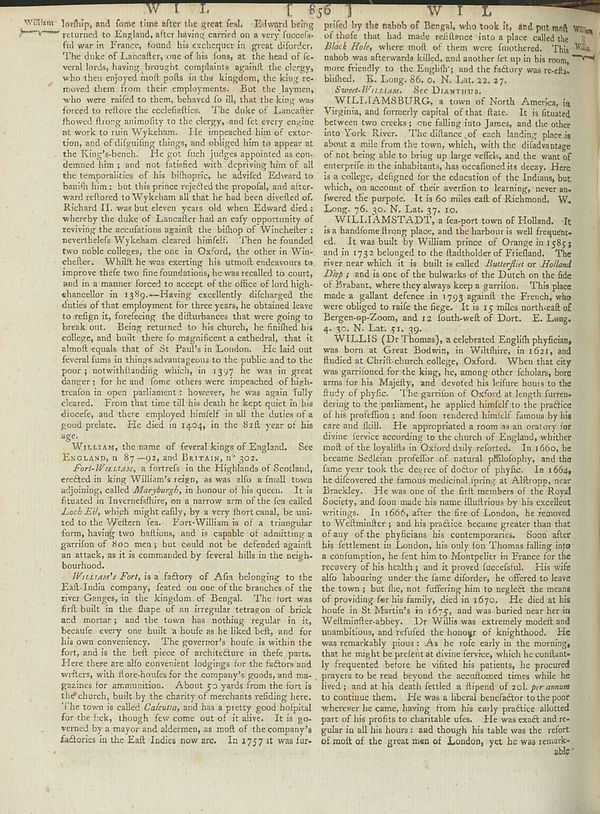
\includegraphics[width=0.85\textwidth]{../scans/page-0258-631a7ae7df34.jpg}
\caption*{Source scan: \texttt{page-0258-631a7ae7df34.jpg}}
\end{figure}

\end{document}
